% ============================================================
%  BAB 2 – TINJAUAN LITERATUR
%  Compile standalone:  pdflatex bab-2.tex
%  Compile as part of thesis: pdflatex main.tex
% ============================================================
\documentclass[main]{subfiles}

\begin{document}

% When standalone: set counter so \chapter{} renders as "BAB 2".
% When in main.tex: main.tex sets the counter before \subfile{bab-2}.
\ifSubfilesClassLoaded{}{\setcounter{chapter}{1}}

\chapter{Tinjauan Literatur}

Bab ini menyajikan landasan konseptual penelitian, mencakup: konsep
dasar \textit{Knowledge Graph} (KG) dan ontologi pendidikan; mekanisme
\textit{Knowledge Graph Completion} (KGC) berbasis \textit{embedding}
maupun LLM; peran LLM sebagai penilai (\textit{LLM-as-a-judge}); metrik
evaluasi KG yang digunakan; konteks interkoneksi kurikulum sains; serta
tinjauan penelitian terkait guna memperjelas posisi dan kontribusi
penelitian ini.

% ============================================================
\section{Landasan Teori}
% ============================================================

\subsection{Knowledge Graph (KG) dan Ontologi Pendidikan}
\label{subsec:kg-ontologi}

Sebagaimana diperkenalkan pada Bab~1, \textit{Knowledge Graph} (KG) merupakan
paradigma representasi pengetahuan yang kini banyak digunakan. Secara formal,
\textcite{hogan_knowledge_2022} mendefinisikan KG sebagai graf data yang
dirancang untuk menghimpun dan merepresentasikan pengetahuan dunia nyata, dengan
simpul (\textit{nodes}) sebagai representasi entitas dan sisi (\textit{edges})
sebagai representasi relasi semantik antarentitas. Informasi dalam KG
diformalkan dalam bentuk triple (\textit{head, relation, tail}) sehingga
hubungan antarinformasi dapat diproses dan ditelusuri secara komputasional oleh
mesin.

Pemaknaan relasi pada KG dapat dipertajam dengan menggunakan tipe relasi
spesifik alih-alih label generik. Sebagai ilustrasi pada domain sains SMA,
sebuah KG dapat merepresentasikan keterkaitan intra-disiplin melalui triple
seperti (Fotosintesis, \texttt{MENGHASILKAN}, Glukosa), sekaligus menjembatani
keterkaitan lintas-disiplin yang sering bersifat implisit, misalnya
(Potensial Elektrode, \texttt{APLIKASI\_DARI}, Potensial Listrik) yang menautkan
Kimia dengan Fisika, serta (DNA, \texttt{PRASYARAT\_UNTUK}, Gen) yang menautkan
Kimia dengan Biologi. Setiap triple menyatakan satu fakta atomik yang secara
kolektif membentuk struktur KG untuk menelusuri keterkaitan lintas konsep.

Dalam konteks pendidikan, \textcite{abu-salih_systematic_2024} dalam tinjauan
sistematisnya menegaskan bahwa KG saat ini mendominasi inovasi teknologi
pembelajaran modern, karena kemampuannya yang sangat transformatif untuk
mendukung pembelajaran adaptif (\textit{adaptive learning}), perancangan
kurikulum berbasis data, serta pemetaan konsep secara visual. Penggunaan
KG memungkinkan sistem untuk menyusun jaringan informasi yang
mencerminkan kerumitan konten kurikulum secara komputasional.

Representasi pengetahuan berbasis KG tidak akan memberikan manfaat
pedagogis yang optimal tanpa kerangka semantik yang mengatur struktur
dan batas maknanya. \textcite{studer_knowledge_1998}, yang memperluas
gagasan \textcite{gruber_translation_1993}, mendefinisikan ontologi sebagai
spesifikasi formal dan eksplisit atas sebuah konseptualisasi bersama terhadap
suatu domain. Kehadiran ontologi pendidikan menjadi penting
karena berfungsi sebagai skema formal yang mendefinisikan jenis entitas
(kelas), jenis relasi (properti), serta aturan keterhubungan dalam suatu
domain. Dalam kerangka KG, ontologi berperan sebagai
\textit{blueprint} yang mengatur struktur graf sehingga setiap triple
yang ditambahkan mengikuti aturan yang konsisten dan dapat
diinterpretasikan mesin secara tepat. Sebagai ilustrasi, ontologi
pendidikan dapat mendefinisikan kelas seperti Konsep, Materi, dan
Disiplin, serta relasi seperti prasyaratDari, bagianDari, dan
terhubungDengan, sehingga triple seperti (Fotosintesis, prasyaratDari,
Respirasi Seluler) menjadi valid dan bermakna secara ontologis.
\textcite{zhang_learning_2023} menunjukkan bahwa dalam konteks silabus dan
\textit{learning path}, konsep pembelajaran dapat direpresentasikan
sebagai entitas spesifik yang dihubungkan melalui relasi ketergantungan
seperti \textit{predecessor} sebagai pengetahuan prasyarat dan
\textit{successor} sebagai pengetahuan lanjutan, sehingga tanpa
struktur ontologis semacam ini, graf yang dihasilkan hanya akan menjadi
kumpulan node dan edge tanpa makna pedagogis yang dapat diandalkan.

Urgensi ontologi ini diperkuat oleh \textcite{guo_ontology-enhanced_2025} yang menegaskan
bahwa sistem ekstraksi pengetahuan berbasis kecerdasan buatan (AI) yang
tidak dipandu oleh ontologi sangat rentan menghasilkan
\textit{hallucination}, yakni pemetaan relasi yang keliru atau tidak
relevan secara keilmuan. Tanpa pengetahuan ontologis yang mendefinisikan
batasan secara eksplisit, sistem AI tidak memiliki panduan normatif
untuk memilih relasi yang valid secara epistemologis. Dalam penelitian
ini, ontologi pendidikan diperlakukan sebagai fondasi wajib yang
menjamin bahwa KG yang dihasilkan memiliki relevansi pedagogis,
konsistensi semantik, dan akurasi keilmuan yang dapat
dipertanggungjawabkan dalam konteks kurikulum sains SMA.

\begin{figure}[htbp]
  \centering
  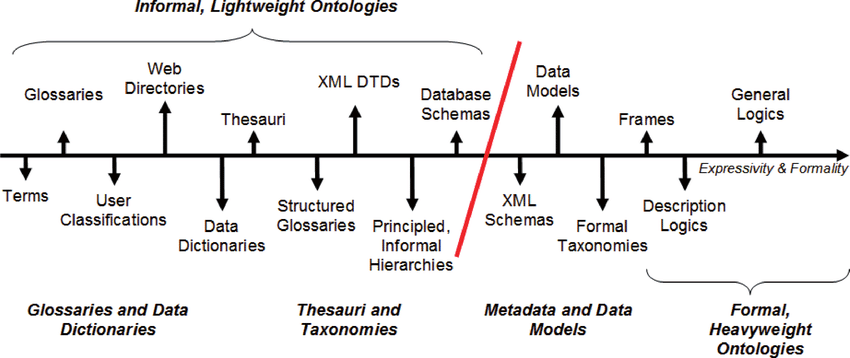
\includegraphics[width=0.9\textwidth]{images/media/image19.png}
  \caption{Spektrum Formalitas Ontologi (diadaptasi dari \textcite{uschold_ontologies_2004})}
  \label{fig:spektrum-ontologi}
\end{figure}

Mengacu pada spektrum formalitas ontologi yang dikemukakan
\textcite{uschold_ontologies_2004} (Gambar~\ref{fig:spektrum-ontologi}),
penelitian ini mengadopsi pendekatan ontologi informal yang berfokus
pada pemodelan hierarki taksonomi konseptual. Pendekatan ini dipilih
karena relevansinya dengan realitas pedagogis saat ini. Berbeda dengan
domain lain seperti kesehatan atau keuangan yang telah banyak mengadopsi
ontologi formal, bidang pendidikan secara historis ditandai oleh
ekosistem yang sangat beragam, sehingga belum memiliki ontologi maupun
skema formal yang diterima secara universal. Pendekatan informal yang
fleksibel namun tetap terstruktur secara hierarkis merupakan solusi yang
lebih pragmatis dan sesuai dengan karakteristik domain ini. Secara konkret,
ontologi yang dirancang dalam penelitian ini berbentuk hierarki taksonomi
konsep, dari mata pelajaran, bab, dan subbab hingga konsep, yang dilengkapi
vokabulari relasi semantik intra- maupun lintas-disiplin; rancangan lengkapnya,
meliputi definisi kelas, relasi objek, dan properti data, dijabarkan pada
Subbab~\ref{subsec:skema-ontologi}.

\subsection{Knowledge Graph Completion}
\label{subsec:kgc}

Setiap KG memiliki keterbatasan inheren berupa sifatnya yang tidak pernah
benar-benar lengkap (\textit{incompleteness}); sebagian relasi yang valid
selalu luput terpetakan ketika graf dibangun. \textit{Knowledge Graph
Completion} (KGC) merupakan tugas komputasional yang mengatasi keterbatasan
ini, yakni menginferensi dan memprediksi entitas atau relasi yang hilang
(\textit{missing links}) agar triple pengetahuan menjadi lebih utuh dan
konsisten secara semantik.

Metode-metode berbasis \textit{embedding} seperti TransE
\parencite{bordes_translating_2013} dan RotatE \parencite{sun_rotate_2019} memodelkan relasi sebagai operasi
matematis dalam ruang vektor berdimensi rendah. Meskipun efisien pada
graf yang padat, seluruh metode dalam keluarga ini mengalami kendala
yang sama: kedekatan antarentitas dikalkulasikan semata-mata berdasarkan
struktur topologi graf, tanpa mempertimbangkan informasi tekstual atau
kontekstual yang melingkupinya \parencite{ji_survey_2022}. Keterbatasan ini
menjadi sangat menonjol pada \textit{long-tail entities} (entitas dengan
konektivitas relasional minim). \textcite{wei_kicgpt_2023} membuktikan secara empiris
bahwa metode \textit{embedding} berbasis triple mengalami degradasi
performa yang signifikan dalam skenario ini karena representasi vektor
entitas yang jarang terhubung tidak cukup terlatih untuk menghasilkan
inferensi yang valid.

Persoalan ini berdampak langsung pada domain pendidikan sains: relasi
lintas-disiplin antara Fisika, Kimia, dan Biologi jarang tersurat dalam
satu sumber teks sehingga secara struktural tergolong \textit{long-tail},
dan karenanya paling sulit ditemukan oleh metode \textit{embedding}
konvensional \parencite{wei_kicgpt_2023}.

Untuk mengatasi keterbatasan tersebut, paradigma KGC modern bergeser menuju pendekatan berbasis
bahasa alami. Alih-alih menghitung jarak spasial, \textcite{yao_exploring_2025}
mereformulasikan KGC sebagai tugas \textit{question answering}: dengan
memperlakukan triple sebagai urutan teks, model diminta menjawab pertanyaan
seperti ``apa yang berhubungan dengan entitas X melalui relasi R?''
berdasarkan pemahaman konteks bahasa. Reformulasi inilah yang membuka jalan
bagi integrasi \textit{Large Language Models} (LLM) ke dalam \textit{pipeline} KGC,
yang menjadi inti kontribusi teknis penelitian ini.

Kapasitas semantik tersebut menghadirkan tantangan komputasional
tersendiri: penerapan LLM secara langsung untuk mengevaluasi seluruh
kandidat relasi dalam graf berskala besar tidaklah praktis. Pencarian
berbasis kemiripan secara menyeluruh (\textit{brute-force}) menghasilkan
kompleksitas waktu $O(n^2)$ yang tidak skalabel, serta berpotensi
terhambat oleh \textit{input token limit} pada arsitektur model bahasa.
Arsitektur KGC modern karenanya memanfaatkan teknologi basis data vektor
atau algoritma \textit{Approximate Nearest Neighbor} (ANN), yang
memungkinkan pencarian kandidat relasi dengan kedekatan semantik
tertinggi secara jauh lebih efisien sebelum dievaluasi lebih lanjut oleh
LLM.

Kedekatan semantik antarvektor tersebut lazim diukur dengan \textit{cosine
similarity}, yaitu kosinus sudut antara dua vektor $\mathbf{a}$ dan $\mathbf{b}$:
\[
  \text{sim}(\mathbf{a}, \mathbf{b})
  = \frac{\mathbf{a} \cdot \mathbf{b}}{\|\mathbf{a}\|\,\|\mathbf{b}\|}
  = \frac{\sum_{i=1}^{d} a_i b_i}
         {\sqrt{\sum_{i=1}^{d} a_i^{2}}\;\sqrt{\sum_{i=1}^{d} b_i^{2}}}.
\]
Pembilang $\mathbf{a} \cdot \mathbf{b} = \sum_{i=1}^{d} a_i b_i$ adalah hasil
kali titik (\textit{dot product}) kedua vektor, sedangkan penyebut merupakan
hasil kali \textit{Euclidean norm} ($L_2$) masing-masing vektor; di sini $d$ menyatakan
dimensi \textit{embedding}, serta $a_i$ dan $b_i$ adalah komponen ke-$i$ dari
$\mathbf{a}$ dan $\mathbf{b}$. Pembagian dengan kedua norma menormalkan panjang
vektor sehingga ukuran ini hanya bergantung pada arah, bukan magnitudo.
Nilainya berada pada rentang $[-1, 1]$; semakin tinggi nilainya, semakin dekat
arah (dan dengan demikian makna) kedua vektor, sehingga untuk \textit{embedding}
teks nilainya umumnya berada pada rentang $[0, 1]$.

Salah satu implementasi ANN yang banyak digunakan pada basis data vektor
modern adalah algoritma \textit{Hierarchical Navigable Small World} (HNSW)
\parencite{malkov_efficient_2020}. HNSW membangun struktur graf berlapis
(\textit{multi-layer navigable graph}) di mana lapisan teratas berisi sedikit
node dengan koneksi jarak jauh (\textit{long-range links}) dan lapisan
terbawah berisi seluruh node dengan koneksi lokal. Pencarian dilakukan
secara \textit{greedy} dari lapisan teratas ke bawah: pada tiap lapisan,
algoritma bergerak ke tetangga yang paling dekat dengan \textit{query}
hingga tidak ada perbaikan, lalu turun ke lapisan berikutnya dengan lebih
banyak node. Pendekatan berlapis ini menurunkan kompleksitas pencarian
per-\textit{query} dari $O(n)$ pada \textit{brute-force} menjadi
$O(\log n)$ rata-rata,
menjadikan HNSW pilihan utama untuk pencarian kemiripan semantik pada
graf pengetahuan berskala besar tanpa mengorbankan akurasi secara
signifikan. Ilustrasi struktur graf berlapis HNSW tersebut ditunjukkan pada
Gambar~\ref{fig:hnsw}.

\begin{figure}[htbp]
  \centering
  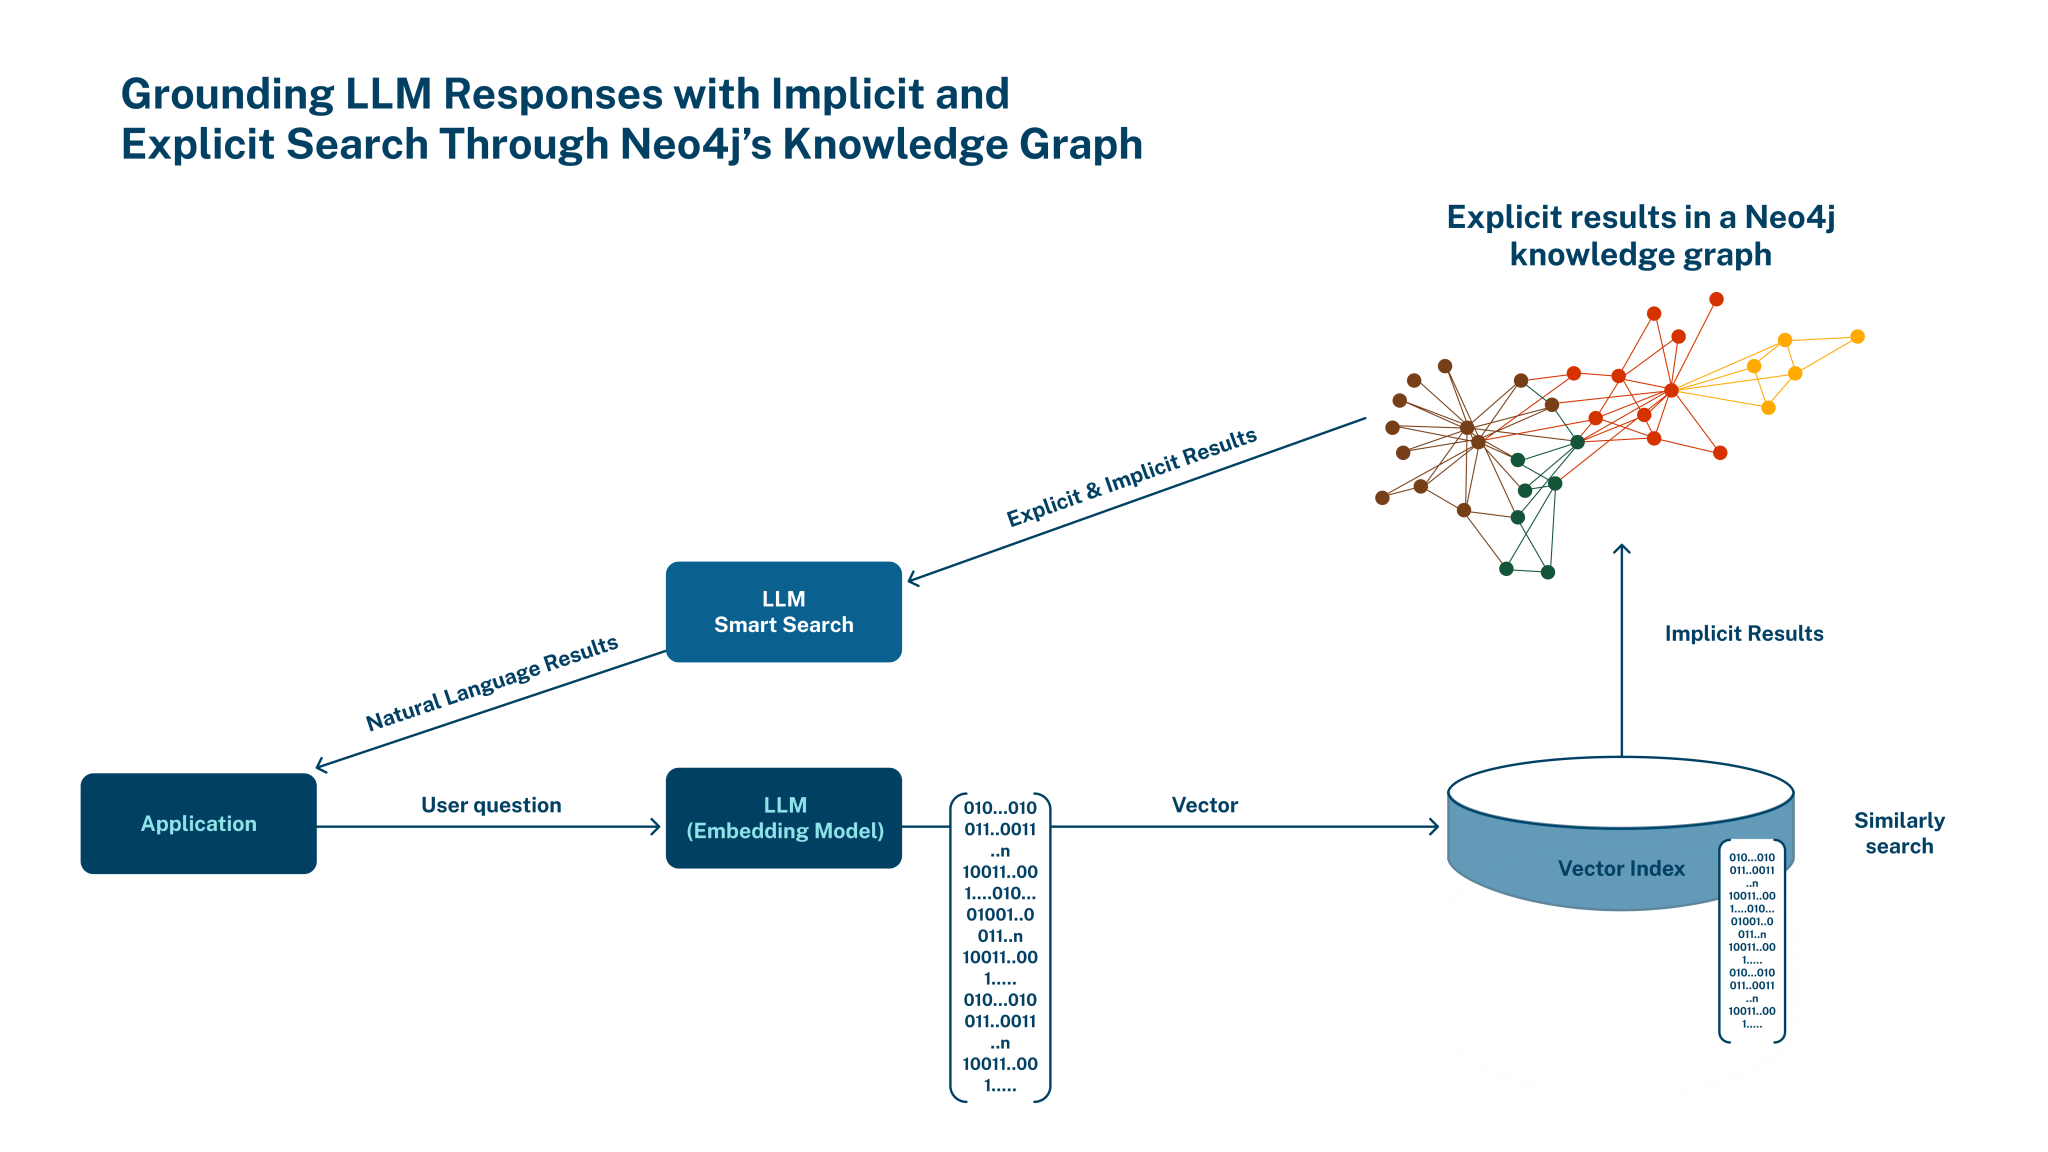
\includegraphics[width=\maxwidth]{images/media/image23.png}
  \caption{Ilustrasi struktur graf berlapis HNSW
  (diadaptasi dari \textcite{malkov_efficient_2020}).}
  \label{fig:hnsw}
\end{figure}

\subsection{Large Language Models (LLM) dan Sinergi LLM-KG}

Perkembangan \textit{Large Language Models} (LLM) telah mendorong
pergeseran paradigma dalam ekosistem kecerdasan buatan, khususnya dalam
hubungannya dengan teknologi KG. \textcite{pan_unifying_2024} memetakan sinergi
antara LLM dan KG ke dalam tiga kerangka konseptual utama:
\textit{KG-enhanced LLMs} (KG digunakan sebagai sumber fakta terstruktur
untuk meningkatkan akurasi dan faktualitas LLM---yakni kesesuaian keluaran
model dengan fakta yang benar sehingga menekan \textit{hallucination}),
\textit{LLM-augmented KGs} (LLM dimanfaatkan untuk
menyelesaikan tugas-tugas konstruksi dan penalaran KG), serta
\textit{Synergized LLMs + KGs} (keduanya beroperasi secara resiprokal
dan setara). Penelitian ini secara spesifik beroperasi dalam kerangka
\textit{LLM-augmented KGs}: kapasitas generalisasi semantik LLM
dimanfaatkan untuk menyempurnakan proses konstruksi graf dan KGC,
khususnya dalam menangkap relasi interdisipliner yang tidak tersurat
secara eksplisit dalam kurikulum.

Sinergi ini secara fundamental mengubah arsitektur kerja KGC
tradisional. \textcite{bian_llm-empowered_2025} mencatat bahwa proses ekstraksi dan
konstruksi KG kini bergeser dari pendekatan statistik-simbolik yang
deterministik dan kaku menuju kerangka berbasis model bahasa generatif
yang lebih adaptif dan \textit{context-sensitive}. Pendekatan deterministik
bertumpu pada aturan eksplisit buatan manusia, seperti pencocokan pola
sintaksis (\textit{regular expression}), \textit{rule-based dependency
parsing}, atau template relasi yang telah ditetapkan. Aturan semacam itu
rapuh terhadap variasi bahasa: untuk mengekstraksi relasi prasyaratDari,
misalnya, sistem harus dibekali pola eksplisit seperti ``untuk memahami X,
siswa perlu menguasai Y'', sehingga ketika gagasan yang sama diungkapkan
sebagai ``Y merupakan fondasi bagi X'' relasi tersebut gagal terdeteksi.
Kekakuan inilah yang membuat pendekatan deterministik sulit menangkap
relasi implisit dan variasi ekspresi bahasa alami yang justru lazim dalam
teks pendidikan.

Keterbatasan serupa tidak hanya berlaku pada metode berbasis aturan,
tetapi juga pada metode \textit{embedding} konvensional yang pengambilan
keputusannya hanya bergantung pada pola koneksi yang telah ada dalam
graf (sebagaimana telah diuraikan sebelumnya). Pergeseran menuju
penggunaan LLM mendefinisikan ulang mekanisme penalaran dalam KGC,
karena LLM mampu memanfaatkan pengetahuan internal yang diperoleh dari
pelatihan pada korpus teks berskala masif untuk mengevaluasi kelayakan
semantik suatu fakta baru, termasuk pada entitas \textit{long-tail} yang
memiliki sedikit koneksi dalam graf \parencite{yao_exploring_2025, wei_kicgpt_2023}.

Salah satu implementasi paling representatif dari paradigma ini adalah
kerangka kerja KICGPT \parencite{wei_kicgpt_2023}, yang memadukan \textit{pipeline} KGC
dengan kemampuan penalaran LLM melalui strategi \textit{In-Context
Learning} (ICL). Inti dari strategi ini adalah mekanisme yang disebut
\textit{Knowledge Prompt}: struktur ontologi KG, termasuk entitas,
relasi, dan batasan semantiknya, dikodekan sebagai demonstrasi teks di
dalam instruksi (\textit{prompt}), sehingga LLM memperoleh panduan
kontekstual yang cukup untuk melakukan \textit{ranking} kandidat relasi
tanpa memerlukan proses \textit{fine-tuning} yang secara komputasional
mahal. Pendekatan ini relevan secara praktis untuk penelitian ini, karena
memungkinkan pemanfaatan LLM dalam skala penelitian akademis tanpa
bergantung pada infrastruktur pelatihan model berskala industri.

\begin{figure}[htbp]
  \centering
  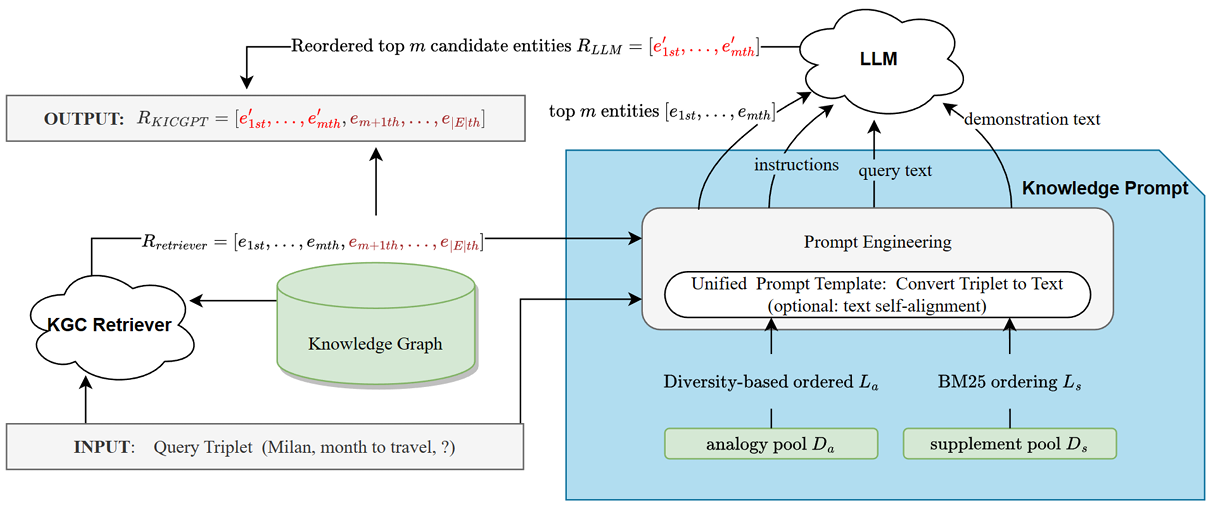
\includegraphics[width=0.85\textwidth]{images/media/image15.png}
  \caption{Ilustrasi Kerangka KICGPT (diadaptasi dari \textcite{wei_kicgpt_2023})}
  \label{fig:kicgpt}
\end{figure}

Untuk merangkum pergeseran paradigma yang telah diuraikan,
Tabel~\ref{tab:kgc-comparison} menyajikan perbandingan konseptual antara
metode KGC konvensional berbasis \textit{embedding} dengan pendekatan
mutakhir yang dibantu LLM, mencakup dimensi sumber data, konteks
penalaran, skalabilitas, serta penanganan \textit{long-tail entities}.

\begin{longtable}{@{}p{0.18\linewidth}p{0.38\linewidth}p{0.38\linewidth}@{}}
  \caption{Perbandingan Metode KGC Tradisional dan LLM-Assisted}
  \label{tab:kgc-comparison}\\
  \toprule
  \textbf{Aspek}
    & \textbf{Metode Tradisional (Pre-2021)}
    & \textbf{Metode LLM-Assisted (2021--Sekarang)} \\
  \midrule
  \endfirsthead
  \toprule
  \textbf{Aspek}
    & \textbf{Metode Tradisional (Pre-2021)}
    & \textbf{Metode LLM-Assisted (2021--Sekarang)} \\
  \midrule
  \endhead
  \midrule
  \endfoot
  \bottomrule
  \endlastfoot
  Sumber Data
    & Terstruktur (RDF/SQL/Simbolik)
    & Tidak Terstruktur (Buku Teks, Modul, Silabus) \\
  Konteks
    & Terbatas pada jarak struktur graf matematis murni
    & Memahami semantik bahasa alami dan konteks teks lintas dokumen \\
  Skalabilitas
    & Membutuhkan intervensi pakar secara masif
    & Ekstraksi otomatis dan generatif dengan verifikasi (ICL) \\
  Penanganan \textit{Long-tail}
    & Performa turun drastis pada data minim koneksi
    & Lebih \textit{robust} dengan memanfaatkan \textit{pre-trained knowledge}
      LLM \\
\end{longtable}

\subsection{Large Language Model sebagai Penilai (LLM-as-a-judge)}

Dalam \textit{pipeline} KGC berbasis LLM, validasi oleh pakar manusia
(\textit{expert-driven evaluation}) merupakan \textit{gold standard}
untuk memastikan kebenaran faktual berkat kedalaman pemahaman
kontekstualnya. Meski demikian, dalam proses anotasi data, tahapan
validasi ini sering kali memunculkan perbedaan pendapat
(\textit{disagreement}) di antara para pakar akibat tingkat
subjektivitas masing-masing penilai \parencite{gu_survey_nodate, zheng_judging_2023}. Untuk mengatasi ketidaksepakatan tersebut tanpa mengorbankan
skalabilitas dan menekan biaya operasional, pemanfaatan LLM dapat
diimplementasikan melalui pendekatan \textit{LLM-as-a-judge}. Dalam skenario ini,
alih-alih difungsikan sebagai penilai utama yang menggantikan peran
manusia, LLM diposisikan secara spesifik sebagai moderator yang objektif
untuk menyelesaikan konflik penilaian antarpakar \parencite{gu_survey_nodate}.

Meskipun terbukti efektif sebagai penengah, literatur menunjukkan bahwa
LLM memiliki kerentanan terhadap bias kognitif saat dihadapkan pada dua
argumen yang berseberangan. Model sering kali terpengaruh oleh
\textit{concreteness bias}, yaitu kecenderungan memihak pada respons
yang menyajikan detail spesifik atau dikemas dengan gaya bahasa yang
meyakinkan, sekalipun argumen tersebut secara faktual keliru
\parencite{gu_survey_nodate, zheng_judging_2023}.

Untuk menjamin reliabilitas keputusan dan menekan tingkat \textit{hallucination}
saat model melakukan arbitrase, proses penengahan oleh LLM menuntut
adanya mekanisme penjangkaran (\textit{grounding}) yang kuat. Sejalan
dengan rekomendasi \textcite{gu_survey_nodate} dan prinsip evaluasi presisi
faktual dari \textcite{min_factscore_2023}, penerapan \textit{LLM-as-a-judge} harus
diiringi dengan injeksi konteks berupa bukti eksternal
(\textit{textbook evidence}). Melalui integrasi referensi buku teks
kurikulum, landasan keputusan tidak lagi bergantung pada asumsi
parametrik internal model yang rentan bias, melainkan berakar pada
kebenaran fakta keilmuan yang disediakan.

% ============================================================
\section{Metrik Evaluasi Knowledge Graph}
% ============================================================

Evaluasi kualitas Knowledge Graph (KG) merupakan aspek krusial dalam
mengukur keberhasilan sistem ekstraksi dan penyelesaian graf yang
dibangun. \textcite{xue_knowledge_2022} menegaskan bahwa evaluasi kualitas tidak
hanya bergantung pada karakteristik bawaan data---yakni akurasi
(kebenaran fakta yang direpresentasikan), konsistensi (ketiadaan
kontradiksi logis antar-triple maupun pelanggaran batasan ontologi), dan
kelengkapan intrinsik (sejauh mana graf memuat seluruh fakta dan relasi
yang seharusnya ada)---tetapi juga krusial untuk
memastikan kredibilitas graf tersebut saat diimplementasikan pada
aplikasi turunannya. Untuk mencapai evaluasi yang komprehensif, metrik
evaluasi KG dalam penelitian ini dikategorikan menjadi tiga kelompok
utama: metrik topologi graf dan metrik ekstraksi---yang mengacu pada metrik kualitas 
struktural \parencite{seo_structural_2022}---serta metrik hubungan antar-entitas yang 
dikembangkan dalam penelitian ini.

\subsection{Metrik Topologi Graf}
\label{subsec:metrik-topologi}

Evaluasi berbasis topologi graf berfokus pada pengukuran karakteristik
fisik dan distribusi relasi jaringan matematis tanpa memandang makna
semantik dari ontologi. \textcite{seo_structural_2022} mengklasifikasikan
perhitungan statistik dasar jaringan seperti kohesi dan kardinalitas ke
dalam kategori metrik graf. Metrik ini sangat krusial untuk memetakan
bagaimana konsep-konsep materi sains berinteraksi satu sama lain secara
struktural. Dalam penelitian ini, analisis topologi graf diukur
menggunakan tiga indikator utama.

\subsubsection{Average Degree Centrality (ADC)}

\textbf{Average Degree Centrality (ADC)} digunakan untuk mengukur
rata-rata jumlah koneksi yang dimiliki oleh setiap simpul
(\textit{node}) dalam graf:

\[
  ADC = \frac{1}{|V|} \sum_{v \in V} \deg(v)
\]

\noindent dengan $|V|$ adalah jumlah simpul dalam graf dan $\deg(v)$
adalah jumlah relasi yang terhubung langsung ke simpul $v$.

Dalam penelitian ini, ADC dihitung dalam dua bentuk. ADC \textbf{graf
keseluruhan} menghitung seluruh simpul dan relasi dalam basis data graf,
termasuk simpul struktural seperti kelas, bab, subbab, konsep, serta
target konsep. ADC \textbf{antar-konsep} hanya melibatkan simpul konsep
dan relasi langsung antar-konsep, merepresentasikan tingkat
keterhubungan konseptual antarmateri sains tanpa dipengaruhi oleh simpul
struktural. ADC antar-konsep digunakan sebagai metrik utama untuk
membandingkan graf sebelum dan sesudah proses KGC, karena lebih langsung
mencerminkan perubahan interkoneksi materi Fisika, Kimia, dan Biologi.

\subsubsection{Modularity}

\textbf{Modularity ($Q$)} mengukur seberapa baik sebuah graf terbagi
menjadi komunitas-komunitas yang terpisah. Nilai $Q$ berkisar antara
$-0{,}5$ hingga $1$; nilai yang lebih tinggi menunjukkan pembagian
komunitas yang lebih baik, ditandai dengan koneksi yang rapat di dalam
komunitas dan jarang di luar komunitas. Nilai $Q = 0$ menunjukkan bahwa
pembagian komunitas yang dihasilkan tidak lebih baik dari partisi acak.

Modularity dihitung dengan membandingkan jumlah \textit{edge} yang
benar-benar ada dalam komunitas dengan jumlah \textit{edge} yang secara
statistik diharapkan muncul apabila koneksi antarsimpul disebar secara
acak---dengan syarat distribusi \textit{degree} tiap simpul
dipertahankan. Untuk graf berarah (\textit{directed graph}), modularity
didefinisikan sebagai:

\[
  Q = \frac{1}{m} \sum_{i} \sum_{j}
      \left[ A_{ij} - \frac{k_i^{\text{out}} \, k_j^{\text{in}}}{m}
      \right] \delta(c_i, c_j)
\]

\noindent dengan:

\begin{itemize}
  \item $A_{ij}$: matriks adjasensi; bernilai 1 jika terdapat
        \textit{edge} dari node $i$ ke node $j$, dan 0 jika tidak ada.
  \item $k_i^{\text{out}}$: \textit{out-degree} dari node $i$.
  \item $k_j^{\text{in}}$: \textit{in-degree} dari node $j$.
  \item $m$: total jumlah \textit{edge} berarah.
  \item $\delta(c_i, c_j) = 1$ jika simpul $i$ dan $j$ berada dalam
        komunitas yang sama; 0 jika tidak.
\end{itemize}

Rumus di atas dapat diekspresikan dalam bentuk yang lebih ringkas dengan
menjumlahkan langsung per komunitas:

\[
  Q = \sum_{c} \left[
      \frac{e_{cc}}{m} - \frac{k_c^{\text{out}} \, k_c^{\text{in}}}{m^2}
      \right]
\]

\noindent dengan $e_{cc}$ adalah jumlah \textit{edge} internal komunitas
$c$, sedangkan $k_c^{\text{out}}$ dan $k_c^{\text{in}}$ adalah total
\textit{out-degree} dan \textit{in-degree} seluruh node dalam komunitas
$c$. Kedua bentuk rumus menghasilkan nilai yang identik; perbedaannya
hanya pada cara penjumlahan.

Dalam penelitian ini, partisi komunitas $c$ ditetapkan secara tetap
berdasarkan mata pelajaran (Fisika, Kimia, dan Biologi), bukan
hasil deteksi komunitas otomatis (Contoh: algoritma \textit{Louvain}).
Penetapan partisi yang tetap ini penting karena nilai $Q$ pre-KGC dan
post-KGC dihitung atas partisi yang persis sama, sehingga perubahan $Q$
murni mencerminkan bertambahnya \textit{edge} lintas-mata-pelajaran akibat
proses KGC, bukan artefak dari komunitas yang berbeda di tiap fase.

\subsubsection{Graph Density}

\textbf{Graph Density ($D$)} mengukur seberapa banyak koneksi yang
terbentuk dalam sebuah graf dibandingkan dengan koneksi maksimum yang
secara teoritis mungkin ada. Nilai $D$ berkisar antara 0 hingga 1; nilai
mendekati 1 menandakan graf yang sangat padat (\textit{dense}), sementara
nilai mendekati 0 menandakan graf yang jarang (\textit{sparse}). Dalam
konteks penelitian ini, \textit{density} digunakan untuk membandingkan tingkat
keterkaitan antar-konsep sebelum dan sesudah penambahan relasi lintas
buku (\textit{cross-book links}). Untuk graf berarah, formula yang
digunakan adalah:

\[
  D = \frac{|E|}{|V|(|V|-1)}
\]

\noindent dengan $|E|$ adalah jumlah total \textit{edge} yang terbentuk
dalam KG, dan $|V|$ adalah jumlah total node. Penyebut
$|V|(|V|-1)$ merepresentasikan jumlah maksimum \textit{edge} berarah
yang mungkin ada, dari asumsi bahwa setiap pasangan node $(i, j)$ dengan
$i \neq j$ dapat memiliki tepat satu \textit{edge} berarah tanpa
\textit{self-loop}.

\subsection{Metrik Ekstraksi}
\label{subsec:metrik-ekstraksi}

Metrik ekstraksi mengevaluasi kualitas proses ekstraksi entitas dan
atribut dari dokumen sumber.

\subsubsection{Description Completeness (DC)}

\textbf{Description Completeness (DC)} mengukur sejauh mana entitas yang
berhasil diidentifikasi juga memiliki informasi pendukung berupa
deskripsi atau definisi. Dalam konteks materi sains, sebuah entitas
seperti ``Fotosintesis'' atau ``Hukum Ohm'' tidak cukup hanya muncul
sebagai nama---ia harus memiliki deskripsi agar dapat digunakan dalam
proses pembelajaran atau KGC. DC didefinisikan sebagai:

\[
  DC = \frac{\bigl|\{ v \in V : \text{desc}(v) \neq \varnothing \}\bigr|}{|V|}
\]

\noindent dengan $V$ sebagai himpunan seluruh entitas yang diekstraksi
(node bertipe \texttt{:Concept} dan \texttt{:Chapter}), dan $\text{desc}(v)$
sebagai atribut deskripsi dari entitas $v$. Target minimal untuk metrik
ini ditetapkan sebesar $\geq 0{,}90$ (90\%).

\subsubsection{Empty SubKonsep Rate (ESR)}

\textbf{Empty SubKonsep Rate (ESR)} digunakan untuk mengevaluasi
efektivitas dekomposisi struktural dalam Knowledge Graph. Ontologi yang
dikembangkan menerapkan hierarki ketat dari \texttt{:Chapter} ke
\texttt{:Subtopic} hingga ke unit terkecil yaitu \texttt{:Concept}.
Setiap entitas pada tingkat induk (\textit{parent}) seharusnya memiliki
setidaknya satu entitas turunan sebagai hasil dekomposisi materi. ESR
mengukur proporsi entitas induk yang tidak memiliki satu pun entitas
turunan (\textit{child}):

\[
  ESR = \frac{\bigl|\{ k \in K : |SK(k)| = 0 \}\bigr|}{|K|}
\]

\noindent dengan $K$ sebagai himpunan seluruh entitas pada level hierarki
induk (misalnya \texttt{:Subtopic}), dan $|SK(k)|$ sebagai jumlah entitas
turunan dari entitas $k$ yang terhubung melalui relasi hierarkis
\texttt{:HAS\_CONCEPT}.

Metrik ini merujuk pada prinsip \textit{Class Instantiation} yang
dikemukakan oleh \textcite{seo_structural_2022}; menurut prinsip ini, setiap kelas yang
didefinisikan dalam ontologi harus dimanfaatkan secara aktif untuk
menampung data. Dalam konteks kurikulum sains, nilai ESR yang rendah
menjamin bahwa setiap topik besar telah berhasil dipecah menjadi
konsep-konsep operasional, sehingga menghindari adanya ``node buntu''
yang tidak informatif dalam peta pembelajaran. Target maksimal untuk
metrik ini ditetapkan sebesar $\leq 0{,}10$ (10\%).

\subsection{Metrik Hubungan Antar-Entitas}
\label{subsec:metrik-hubungan}

\subsubsection{Typed Relation Ratio (TRR)}

\textbf{Typed Relation Ratio (TRR)} mengukur sejauh mana relasi dalam KG
menggunakan tipe relasi spesifik dari \textit{controlled vocabulary}
ontologi dibandingkan dengan relasi generik. Berdasarkan ontologi yang
didefinisikan, terdapat 20 tipe relasi spesifik yang terbagi menjadi dua
kelompok: intra-buku (15 tipe, seperti \texttt{MENYEBABKAN} atau
\texttt{BERGANTUNG\_PADA}) dan lintas-buku (5 tipe, seperti
\texttt{LINTAS\_BUKU\_APLIKASI\_DARI}).

\[
  TRR = \frac{|T_{\text{typed}}|}{|T_{\text{total}}|}
\]

\noindent dengan $T_{\text{typed}}$ adalah himpunan relasi dalam KG yang
menggunakan tipe relasi spesifik dari \textit{controlled vocabulary}
ontologi, dan $T_{\text{total}}$ adalah jumlah keseluruhan relasi yang
ada di dalam KG.

Nilai TRR yang tinggi menunjukkan bahwa setiap relasi dalam KG
menggunakan tipe relasi spesifik dari ontologi, bukan label generik. Hal
ini membedakan KG yang bersifat \textit{assertional} (sekadar menyatakan
bahwa dua entitas berhubungan) dari KG yang bersifat \textit{explanatory}
(yang mampu menjelaskan jenis hubungan yang ada). Misalnya, relasi
berlabel \texttt{MENYEBABKAN} membawa makna kausalitas yang dapat
ditelusuri, sementara relasi generik tanpa tipe tidak memberikan informasi
semantik tambahan.

\subsection{Validasi Manusia (Human Evaluation)}
\label{subsec:validasi-manusia}

Selain mengandalkan metrik kuantitatif, proses evaluasi KG mutlak
membutuhkan validasi kualitatif oleh pakar terkait. Hal ini penting
mengingat proses KGC dalam penelitian ini dibantu oleh LLM yang rentan
terhadap \textit{hallucination} informasi, seperti mengekstrak entitas yang salah
atau memetakan relasi lintas disiplin yang tidak relevan secara
pedagogis. Dalam evaluasi klasifikasi tradisional, prediksi sistem
dinilai secara biner---hanya ada benar (1,0) atau salah (0,0), yang
disebut sebagai himpunan tegas (\textit{crisp sets}). Sebaliknya, dalam
evaluasi ekstraksi pengetahuan oleh LLM, hasil sering kali memiliki
batas yang tidak tegas (\textit{soft boundaries}) karena adanya nilai
kebenaran parsial \parencite{harju_evaluating_2023}.

Untuk mengakomodasi hal tersebut, penelitian ini mengadopsi metrik Fuzzy
Precision and Recall. Berdasarkan teori himpunan fuzzy, setiap elemen
memiliki nilai keanggotaan (\textit{membership value}) antara 0 hingga 1
yang merepresentasikan derajat kebenarannya \parencite{harju_evaluating_2023}.
Dalam penelitian ini, kategori evaluasi pakar dipetakan ke dalam nilai
keanggotaan fuzzy sebagai berikut:

\begin{itemize}
  \item \textbf{Benar (1,0):} representasi keanggotaan penuh
        (\textit{full membership}); relasi 100\% akurat secara keilmuan.
  \item \textbf{Sebagian Benar (0,5):} representasi keanggotaan parsial;
        relasi mengandung fakta saintifik namun memerlukan perbaikan
        deskripsi.
  \item \textbf{Kurang Konteks (0,25):} informasi teknis ada, namun
        ketiadaan konteks membatasi fungsionalitas relasi dalam graf
        pembelajaran.
  \item \textbf{Salah / Triple Hilang (0,0):} representasi nol
        keanggotaan; relasi keliru secara ontologis atau gagal
        diekstraksi.
\end{itemize}

Untuk menghitung metrik evaluasi ini, \textcite{harju_evaluating_2023} menggunakan
prinsip irisan fuzzy (\textit{fuzzy intersection}) yang didefinisikan
sebagai nilai minimum antara prediksi model dan referensi
\textit{ground truth} pakar, yaitu $\min(\hat{y}_i, y)$. Karena model
LLM selalu menghasilkan prediksi dengan tingkat keyakinan penuh
($\hat{y}_i = 1{,}0$), nilai irisan dari setiap relasi akan selalu
mengikuti skor keanggotaan yang ditetapkan oleh pakar. Dengan demikian,
rumus evaluasi Fuzzy Precision, Fuzzy Recall, dan F1-Score dirumuskan
sebagai berikut:

\begin{enumerate}
  \item \textbf{Fuzzy Precision:} mengukur tingkat akurasi dari
        keseluruhan relasi yang berhasil diekstrak oleh model LLM.
        \[
          \text{Precision} =
          \frac{\text{Benar}
                + 0{,}5 \cdot \text{SebagianBenar}
                + 0{,}25 \cdot \text{KurangKonteks}}
               {\text{Benar}
                + \text{SebagianBenar}
                + \text{KurangKonteks}
                + \text{Salah}}
        \]

  \item \textbf{Fuzzy Recall:} mengukur sejauh mana sistem berhasil
        menangkap seluruh relasi penting yang diwajibkan dalam kurikulum.
        Penyebut merepresentasikan kardinalitas total dari
        himpunan referensi pakar, termasuk relasi yang gagal diekstraksi
        (Hilang).
        \[
          \text{Recall} =
          \frac{\text{Benar}
                + 0{,}5 \cdot \text{SebagianBenar}
                + 0{,}25 \cdot \text{KurangKonteks}}
               {\text{Benar}
                + \text{SebagianBenar}
                + \text{KurangKonteks}
                + \text{Hilang}}
        \]

  \item \textbf{F1-Score:} rata-rata harmonik antara Precision dan Recall
        untuk memberikan representasi kualitas ekstraksi model secara
        keseluruhan.
        \[
          F_1 = 2 \times
          \frac{\text{Precision} \times \text{Recall}}
               {\text{Precision} + \text{Recall}}
        \]
\end{enumerate}

Melalui pendekatan ini, evaluasi kualitatif dari pakar secara langsung
diterjemahkan menjadi indikator performa kuantitatif, sehingga kualitas
dan kelayakan KG untuk diimplementasikan dalam Kurikulum Merdeka dapat
dipertanggungjawabkan secara komputasional maupun pedagogis.

\subsubsection{Pengujian Reliabilitas Pakar (Inter-rater Reliability)}

Untuk memastikan bahwa penentuan validitas suatu relasi sains tidak
didasari oleh bias subjektif individu, evaluasi kualitatif harus
diiringi dengan perhitungan tingkat kesepakatan antarpenilai
(\textit{inter-rater agreement}).

Pada evaluasi sistem LLM, khususnya ketika \textit{output} sistem
diprediksi memiliki akurasi tinggi, distribusi label yang diberikan oleh
pakar cenderung tidak seimbang (\textit{imbalanced}), yaitu ketika satu
kategori (misalnya label ``Benar'') muncul jauh lebih dominan
dibandingkan kategori lainnya. Pada kondisi distribusi yang miring
(\textit{skewed}) seperti ini, metrik konvensional seperti Cohen's Kappa
kurang cocok karena rentan terhadap Kappa Paradox, yaitu fenomena ketika Kappa
cenderung meremehkan tingkat kesepakatan pada skenario yang sangat tidak
seimbang, sehingga menghasilkan skor rendah meskipun kesepakatan aktual
antarpakar sangat tinggi \parencite{gwet_handbook_2014, james_counting_2026}.

Gwet's AC1 mengatasi kelemahan ini dengan estimasi peluang kesepakatan
yang lebih \textit{robust}:

\[
  AC_1 = \frac{P_a - P_e}{1 - P_e}
\]

\noindent dengan $P_a$ adalah proporsi kesepakatan aktual
(\textit{observed agreement}) antarpakar, dan $P_e$ adalah proporsi
kesepakatan yang diharapkan terjadi secara kebetulan (\textit{expected
agreement}), dirumuskan sebagai:

\[
  P_e = \frac{1}{q-1} \sum_{k} \hat{p}_k (1 - \hat{p}_k)
\]

\noindent dengan $q$ adalah jumlah kategori label dan $\hat{p}_k$ adalah
proporsi penilai yang menetapkan label kategori $k$. Rumus $P_e$ inilah
yang membedakan Gwet's AC1 dari Kappa: estimasi peluang kesepakatan
dihitung berdasarkan proporsi penggunaan kategori secara aktual, sehingga
nilai AC1 tetap mencerminkan kesepakatan yang sesungguhnya meskipun satu
label muncul jauh lebih sering daripada label lainnya
\parencite{mahbub_multi-stage_2026}.

Nilai AC1 berada pada rentang $-1$ hingga $1$, dengan kategori
interpretatif sebagai berikut: buruk ($<0{,}40$), sedang
($0{,}40$--$0{,}60$), baik ($0{,}60$--$0{,}80$), dan sangat baik
($>0{,}80$).

% ============================================================
\section{Interkoneksi Materi Sains dalam Konteks Kurikulum Merdeka}
% ============================================================

Sebagaimana diuraikan pada Bab~1, penerapan Kurikulum Merdeka di jenjang
SMA Fase~F masih menghadapi kesenjangan struktural antara filosofi
pembelajaran lintas-disiplin dan realitas tiga mata pelajaran IPA yang
terpisah secara administratif. Kesenjangan ini secara tidak langsung
merupakan masalah representasi pengetahuan: relasi-relasi
interdisipliner yang ada dalam sains tidak pernah dikodifikasi secara
eksplisit dalam dokumen kurikulum. Sebagai respons pedagogis, pendekatan
pemetaan \textit{Disciplinary Core Ideas} (DCI) dan
\textit{Interdisciplinary Core Ideas} (ICI) telah terbukti menjanjikan:
\textcite{semilarski_expanding_2022} membuktikan bahwa pemetaan visual konsep inti
lintas disiplin sains secara signifikan meningkatkan efikasi diri
(\textit{self-efficacy}) siswa---yaitu keyakinan siswa atas kemampuannya
sendiri dalam memahami sains. Di sisi lain, studi yang sama juga
mengidentifikasi hambatan penting: guru dan siswa mengalami kesulitan
ketika harus memetakan irisan konsep-konsep abstrak secara manual,
terutama antara Fisika dan Kimia. Hambatan ini mengindikasikan bahwa
pendekatan tersebut memerlukan dukungan komputasional agar dapat berjalan
secara efisien.

Kebutuhan akan otomatisasi inilah yang menjadi justifikasi metodologis
inti penelitian ini. Acuan serupa telah diletakkan oleh
\textcite{said_mapping_2024}, yang mengekstraksi kata kunci esensial dari silabus sains dan
matematika untuk memetakan interkoneksinya terhadap Tujuan Pembangunan
Berkelanjutan (SDGs) secara komputasional. Penelitian ini mengadopsi dan
memperluas logika serupa dengan memanfaatkan metode \textit{LLM-Assisted
Knowledge Graph Completion}: konsep-konsep materi sains yang tersebar
dan terisolasi secara struktural diorganisasi ke dalam KG, kemudian LLM
ditugaskan untuk menginferensi relasi interdisipliner yang bersifat
implisit di antara konsep-konsep Fisika, Kimia, dan Biologi.

% ============================================================
\section{Penelitian Terkait}
% ============================================================

Bagian ini memetakan posisi penelitian ini di antara karya-karya
terdahulu yang relevan, mencakup tiga kluster utama: (1) pembangunan KG
berbasis teks pendidikan, (2) KGC berbasis LLM pada domain pengetahuan
umum, dan (3) pemetaan interkoneksi kurikulum secara komputasional.

Pada kluster pertama, \textcite{zhang_learning_2023} mengembangkan KG silabus
berbasis relasi prasyarat untuk mendukung \textit{adaptive learning
path}. Studi tersebut menunjukkan bahwa relasi prasyarat dan \textit{successor}
yang dikodifikasi secara eksplisit secara signifikan meningkatkan
efektivitas rekomendasi urutan belajar. Perbedaan utama dengan penelitian
ini adalah cakupan domain: \citeauthor{zhang_learning_2023} bekerja pada satu mata pelajaran
tunggal, sementara penelitian ini secara spesifik menargetkan relasi
lintas tiga disiplin ilmu (Fisika, Kimia, Biologi) dalam satu kurikulum
nasional yang sama.

Pada kluster kedua, \textcite{wei_kicgpt_2023} mengajukan kerangka KICGPT yang
membuktikan efektivitas ICL berbasis \textit{Knowledge Prompt} untuk KGC pada
dataset umum (FB15k-237 dan WN18RR). Kontribusi teknis \citeauthor{wei_kicgpt_2023}
menjadi fondasi \textit{pipeline} klasifikasi relasi lintas-disiplin dalam
penelitian ini. Perbedaan kritis terletak pada konteks: dataset
\textit{benchmark} \citeauthor{wei_kicgpt_2023} bersifat bahasa Inggris dengan entitas
berupa fakta umum, sedangkan penelitian ini beroperasi pada bahasa
Indonesia dengan entitas berupa konsep kurikulum sains SMA yang
terstruktur secara pedagogis.

Pada kluster ketiga, \textcite{said_mapping_2024} membuktikan kelayakan
otomatisasi pemetaan kurikulum, tetapi pendekatannya terbatas pada analisis
kata kunci tanpa membangun struktur graf relasional. Sementara itu,
\textcite{semilarski_expanding_2022} menunjukkan nilai pedagogis pemetaan
DCI/ICI, tetapi skalabilitasnya terbatas karena dilakukan secara manual.
Penelitian ini mengisi kekosongan tersebut dengan menggabungkan otomatisasi
berbasis LLM dan struktur graf relasional dalam satu \textit{pipeline} yang
terintegrasi, khusus untuk konteks kurikulum Indonesia.

Secara keseluruhan, belum ditemukan penelitian terdahulu yang secara
bersamaan: (a) menggunakan buku teks resmi kurikulum Indonesia sebagai
korpus, (b) membangun KG lintas tiga disiplin IPA dengan ontologi
berbasis OWL, (c) menerapkan LLM-Assisted KGC dengan strategi
\textit{few-shot}, \textit{schema-constrained prompting} untuk ekstraksi
entitas maupun klasifikasi relasi lintas-disiplin, serta (d)
memvalidasi hasilnya menggunakan \textit{pipeline LLM-as-a-judge} berbasis Gemini
dengan metrik \textit{Fuzzy Precision and Recall}. Kombinasi keempat elemen
inilah yang menjadi kontribusi orisinal penelitian ini.

\ifSubfilesClassLoaded{\printbibliography[title={Daftar Pustaka}]}{}

\end{document}
